\documentclass[11pt,a4paper]{ltxdoc}

\usepackage{newtx}
\usepackage[left=1.5in,right=1in,top=1in,bottom=1in]{geometry}
\setlength\parindent{0pt}
\setlength\parskip{.5em}

\usepackage{carom}

\renewcommand\MacroFont{\color{blue}\ttfamily}
\def\bluett#1{{\color{blue}\texttt{#1}}}

\usepackage{booktabs}
\renewcommand{\arraystretch}{1.2}
\setlength\heavyrulewidth{0.16em}

\begin{document}

\title{The \texttt{carom} package}
\author{Anthony Saint-Criq ($s$atplotlib)}
\maketitle

\begin{bTable}[centering]
    \RBall (6,2);
    \YBall (2,2);
    \WBall (2,1.5);
    \Qty[60:.75]{-.5};
    \draw \wpos \To \rbdry[90] \To (7.7,4) -- (8,3.8) \To (5.2,0) \To \ypos;
    \dash \rpos -- (8,1.2) -- (3.7,0) -- (.5,.6);
    \ShadedRegion (0,0) -- (8/3,4);
\end{bTable}

\section{Introduction}

The \bluett{carom} package provides a new environment together with a collection of Tik\textit{Z} macros designed to facilitate the creation of French billiards table diagrams.

French billiards (also known as ``carom billiards'') is played on a pocketless table with only three balls. The objective is to strike the cue ball (either white or yellow, one for each player) so that it subsequently contacts the other two balls. Successfully doing so scores a point and entitles the player to continue their turn until a point is no longer scored.

The cue ball may be struck off-center to impart spin (commonly referred to as an ``effect''). Likewise, the point of contact on the object ball plays a significant role in determining the resulting trajectory.

This package provides tools for indicating ball positions on the table, as well as the intended point of impact on the cue ball and the desired aiming point on the object ball.

The author is grateful to the \TeX\ hackers from Mathcord: Valentin Dao ($x$nkaa) and $q$igamma for reviewing portions of the code, $\gamma$loud for their guidance and explanations, and $x$nkaa again for assistance in sanitizing the source code.

\section{The \bluett{bTable} Environment}

The package defines a \bluett{bTable} environment, which provides the drawing area representing a French billiards table, and defines some commands available for placing and annotating objects on it.

\begin{minipage}{.57\linewidth}
    \begin{bTable}[scale=.9]
        %
    \end{bTable}
\end{minipage}
\begin{minipage}{.43\linewidth}
    \begin{verbatim}
\begin{bTable}[<key=value>]
    % inner code
\end{bTable}
    \end{verbatim}
\end{minipage}\medskip

The optional argument consists of a comma-separated list of \texttt{key=value} pairs controlling various aspects of the diagram.

\begin{macro}{centering}
    This key controls whether the table is horizontally centered with respect to the page layout. Its value defaults to \texttt{false}.
\end{macro}

\begin{macro}{portrait}
    This boolean key selects portrait orientation for the table. When set to \texttt{true}, the table is typeset in portrait mode. When set to \texttt{false} (default), the standard orientation is used.
\end{macro}

\begin{macro}{scale}
    This key is equivalent to Tik\textit{Z}’s \texttt{scale} key and follows the same semantics. It sets a scaling factor applied to the entire table. The value must be a positive floating-point number. A value of \texttt{1} corresponds to the default size, while values greater than \texttt{1} enlarge the table and values between \texttt{0} and \texttt{1} reduce its size. Negative values are not supported.
\end{macro}

\begin{macro}{guidelines}
    This boolean key controls whether auxiliary construction guidelines are displayed on the table. When set to \texttt{true}, the guidelines used for construction and alignment purposes are drawn. When set to \texttt{false} (default), these guidelines are suppressed. These are \textit{not} intended for printing.

    \begin{bTable}[centering,guidelines]
        %
    \end{bTable}

    The guidelines exhibit a coordinate system, which will be described in the next section.
\end{macro}

\begin{macro}{ballsize}
    This key takes a dimension and defaults to \texttt{3pt}. It sets the radius of the balls on the table and updates the \bluett{\textbackslash br} macro accordingly (see the next section). Note that the \bluett{scale} key \textit{does} affect the ball size: \texttt{ballsize=3pt} does not produce a 6pt-wide element in the document unless \texttt{scale=1}.
\end{macro}

\begin{macro}{gridlines}
    This key toggles whether the dotted gridlines should be shown on the table. The default value is \texttt{true}.
\end{macro}

\begin{macro}{cadre,ancres}
    These are boolean keys, both defaulting to \texttt{false}, which control the display of some auxiliary markings on the table. The \bluett{cadre} key enables the display of the ``lignes de cadre'' (for the $42/2$ game), while the \bluett{ancres} key enables the display of the ``ancres'' (for the $47/2$ game). Typically, the ancres are not displayed without the cadre being enabled.
\end{macro}

\begin{macro}{mouches}
    This boolean key controls the display of the side markings (``mouches'') on the table. When set to \texttt{true} (default), the markings are drawn; when set to \texttt{false}, they are suppressed.
\end{macro}

\begin{minipage}{.56\linewidth}
    \begin{bTable}[scale=.86,gridlines=false,cadre,ancres,mouches=false]
        %
    \end{bTable}
\end{minipage}
\begin{minipage}{.44\linewidth}
    \begin{verbatim}
\begin{bTable}[gridlines=false,
    cadre,ancres,mouches=false]
    % inner code
\end{bTable}
    \end{verbatim}
\end{minipage}\bigskip

The default value for each key is summarized in the following table. As is standard for boolean keys, the value may be omitted; in that case, specifying \texttt{[key]} is equivalent to \texttt{[key=true]}. The value \texttt{false} must, however, be stated explicitly, i.e., \texttt{[key=false]} cannot be abbreviated.

\begin{center}
    \begin{tabular}{ccc}
        \toprule
        \textbf{Key} & \textbf{Type} &\textbf{Default value} \\\toprule
        \bluett{centering} & Boolean & \texttt{false} \\\midrule
        \bluett{portrait} & Boolean & \texttt{false} \\\midrule
        \bluett{scale} & Float & \texttt{1.0} \\\midrule
        \bluett{guidelines} & Boolean & \texttt{false} \\\midrule
        \bluett{ballsize} & Dimension & \texttt{3pt} \\\midrule
        \bluett{gridlines} & Boolean & \texttt{true} \\\midrule
        \bluett{cadre} & Boolean & \texttt{false} \\\midrule
        \bluett{ancres} & Boolean & \texttt{false} \\\midrule
        \bluett{mouches} & Boolean & \texttt{true} \\\bottomrule
    \end{tabular}
\end{center}

\section{Commands Available Inside the \bluett{bTable} Environment}

A French billiards table is a rectangle composed of two squares. To draw elements on the table, a coordinate system is used, which can be displayed using the \bluett{guidelines} key. Traditionally, the ``mouches'' are numbered from $1$ to either $3$ or $7$, depending on the side of the table. This is reflected by using coordinates ranging from $0$ to $8$ along the $x$-axis, and from $0$ to $4$ along the $y$-axis.

The package defines many commands that are \textbf{scoped} to the \bluett{bTable} environment.

\begin{macro}{\WBall,\RBall,\YBall,\BBall,\GBall,\KBall,\OBall,\PBall,\VBall,\MBall}
    These commands respectively place the white, red, yellow, blue\footnote{There is a beginner-friendly variant of the game in which a fourth, blue ball is added; in this variant, striking two of the other three balls is sufficient to score a point.}, green, black, orange, pink, violet and maroon balls on the table at the specified coordinates.
    
    Note that no warning is issued if a ball is placed outside the rectangle delimited by the coordinates $(0,0)$ and $(8,4)$.
    
    It is possible not to use any of each ball’s colour-specific macro, as well as to include the same colour of ball multiple times (although this may have undesired consequences; see later).
    
    These macros expect the coordinates of a point, followed by a semicolon (following standard Tik\textit{Z} conventions).\medskip

    \begin{minipage}{.53\linewidth}
        \begin{bTable}[scale=.82]
            \RBall (6,2);
            \YBall (2,2);
            \WBall (2,1.5);
            \BBall (1,2);
            \KBall (3,2);
            \VBall (4,2);
            \GBall (5,2);
            \OBall (7,1);
            \PBall (7,3);
            \MBall (7,2);
            \draw \rpos node[yshift=-.66em,fill=white,inner sep=1pt] {\footnotesize R};
            \draw \wpos node[yshift=-.66em,fill=white,inner sep=1pt] {\footnotesize W};
            \draw \ypos node[yshift=.66em,fill=white,inner sep=1pt] {\footnotesize Y};
            \draw \bpos node[xshift=-.66em,fill=white,inner sep=1pt] {\footnotesize B};
            \draw \kpos node[yshift=-.66em,fill=white,inner sep=1pt] {\footnotesize K};
            \draw \vpos node[yshift=-.66em,fill=white,inner sep=1pt] {\footnotesize V};
            \draw \gpos node[yshift=-.66em,fill=white,inner sep=1pt] {\footnotesize G};
            \draw \opos node[xshift=-.66em,fill=white,inner sep=1pt] {\footnotesize O};
            \draw \ppos node[xshift=-.66em,fill=white,inner sep=1pt] {\footnotesize P};
            \draw \mpos node[xshift=.66em,fill=white,inner sep=1pt] {\footnotesize M};
        \end{bTable}
    \end{minipage}
    \begin{minipage}{.47\linewidth}
        \begin{verbatim}
\begin{bTable}
    \RBall (6,2);    \VBall (4,2);
    \YBall (2,2);    \GBall (5,2);
    \WBall (2,1.5);  \OBall (7,1);
    \BBall (1,2);    \PBall (7,3);
    \KBall (3,2);    \MBall (7,2);
\end{bTable}
        \end{verbatim}
    \end{minipage}
\end{macro}

\begin{macro}{\draw,\dash}
    These commands are used to draw trajectories on the board. The \bluett{\textbackslash draw} command is based on the standard Tik\textit{Z} one, with additional handling to integrate with the package’s layer system. The \bluett{\textbackslash dash} command is provided as a convenience alias for a \texttt{densely dashed} version of \bluett{\textbackslash draw}.
    
    Note that, regardless of where these macros are used in the environment's code, balls will always render \textit{above} all path elements.
\end{macro}

\begin{macro}{\wpos,\rpos,\ypos,[...]}
    When the \bluett{\textbackslash WBall} command is used, the \bluett{\textbackslash wpos} macro stores the coordinates of the white ball. This may subsequently be reused as a shorthand for the ball’s position. The same behaviour applies to the other ball colours provided by the package.
    
    The \bluett{\textbackslash wpos} macro may be used before \bluett{\textbackslash WBall} is called; similarly for the corresponding macros of the other colours. However, if no \bluett{\textbackslash WBall} command has been issued, \bluett{\textbackslash wpos} is not defined, and an \texttt{Undefined control sequence} error is raised. Furthermore, if \bluett{\textbackslash WBall} is used multiple times, only the last specified position is stored in \bluett{\textbackslash wpos}.
\end{macro}\smallskip

\begin{minipage}{.75\linewidth}
    \begin{macro}{\wbdry,\rbdry,\ybdry,[...]}
        In order to facilitate the drawing of trajectories involving collisions, the user may wish to target a point on the boundary of a ball. Consequently, when the \bluett{\textbackslash RBall} command is used, the \bluett{\textbackslash rbdry} macro is defined. It may be used within the syntax of a \bluett{\textbackslash draw} command with a mandatory argument specifying the angle at which the boundary point is taken. For instance, \texttt{\textbackslash rbdry[60]} denotes the point shown in red in the accompanying diagram.\vspace{.5em}
        
        If no \bluett{\textbackslash RBall} command has been issued, calling the \bluett{\textbackslash rbdry} macro results in an \texttt{Undefined control sequence} error.
    \end{macro}
\end{minipage}
\begin{minipage}{.25\linewidth}
    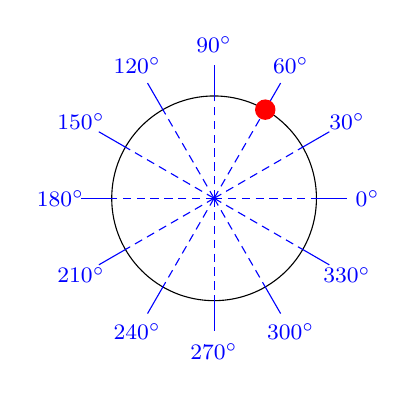
\begin{tikzpicture}[scale=1.3]
        \draw (0,0) circle (1);
        \foreach \i in {0, 30, ..., 330} {
            \draw[blue] ({cos(\i)},{sin(\i)}) -- ({1.3*cos(\i)},{1.3*sin(\i)});
            \draw[blue,densely dashed] (0,0) -- ({cos(\i)},{sin(\i)});
            \draw[blue] ({1.5*cos(\i)},{1.5*sin(\i)}) node {\footnotesize$\i^\circ$};
        }
        \draw[draw=none,fill=red] (60:1) circle (.1);
    \end{tikzpicture}
\end{minipage}

\begin{macro}{\To}
    This may be used in any \bluett{\textbackslash draw} command as a replacement for \texttt{--}, in order to display arrow marks along the middle of the path.
\end{macro}

We now give an example of a diagram, where we display how to perform the game's opening shot.\medskip

\begin{bTable}[centering,scale=1.5]
    \RBall (6,2);
    \YBall (2,2);
    \WBall (2,1.5);
    \draw \wpos \To \rbdry[110] \To (7.7,4) -- (8,3.8) \To (5.2,0) \To \ypos;
    \dash \rpos -- (8,1.2) -- (3.7,0) -- (.5,.6);
\end{bTable}

\begin{verbatim}
\begin{bTable}[centering,scale=1.5]
    \RBall (6,2);
    \YBall (2,2);
    \WBall (2,1.5);
    \draw \wpos \To \rbdry[110] \To (7.7,4) -- (8,3.8)
        \To (5.2,0) \To \ypos;
    \dash \rpos -- (8,1.2) -- (3.7,0) -- (.5,.6);
\end{bTable}
\end{verbatim}

\begin{macro}{\Box,\ShadedRegion,\ShadedBox}
    These macros allow the user to delimit rectangular areas on the table, often indicating where a given set of balls should be located after a shot is played.

    These macros expect two point coordinates, separated by \texttt{--} and terminated by a semicolon, as is standard with Tik\textit{Z} commands.
\end{macro}

\begin{macro}{\blBox,\brBox,\tlBox,\trBox}
    These are aliases for, respectively: \texttt{\textbackslash Box (0,0)--(8/6,4/3)}, \texttt{\textbackslash Box (8-8/6,0)--(8,4/3)}, \texttt{\textbackslash Box (0,4-4/3)--(8/6,4)} and \texttt{\textbackslash Box (8-8/6,4-4/3)--(8,4)}. These aliases \textit{do} expect a semicolon. They allow the user to draw square boxes whose side length is one third of the table width, positioned in each of the four corners.\medskip

    \begin{minipage}{.5\linewidth}
    \centering
        \begin{bTable}[scale=.75]
            \Box (1,1)--(3,3);
        \end{bTable}\par
        \bluett{\textbackslash Box (1,1)--(3,3);}
    \end{minipage}
    \begin{minipage}{.5\linewidth}
    \centering
        \begin{bTable}[scale=.75]
            \ShadedBox (8-8/3,4-2*4/3)--(8,4);
        \end{bTable}\par
        \bluett{\textbackslash ShadedBox (8-8/3,4-2*4/3)--(8,4);}
    \end{minipage}

    \begin{minipage}{.5\linewidth}
    \centering
        \begin{bTable}[scale=.75]
            \tlBox;
        \end{bTable}\par
        \bluett{\textbackslash tlBox;}
    \end{minipage}
    \begin{minipage}{.5\linewidth}
    \centering
        \begin{bTable}[scale=.75]
            \ShadedRegion (2,0) -- (4,1);
        \end{bTable}\par
        \bluett{\textbackslash ShadedRegion (2,0)--(4,1);}
    \end{minipage}\medskip

    In the case where the \bluett{portrait} key is set to \texttt{true}, \bluett{\textbackslash blBox} is \textit{not} placed in the bottom-left corner of the printed document. The \bluett{guidelines} reflect this by indicating the name of each corner.

    \begin{minipage}{.5\linewidth}
        \begin{bTable}[portrait,guidelines]
            \blBox;
        \end{bTable}
    \end{minipage}
    \begin{minipage}{.5\linewidth}
        \begin{verbatim}
\begin{bTable}[portrait,guidelines]
    \blBox;
\end{bTable}
        \end{verbatim}
    \end{minipage}
\end{macro}

\begin{macro}{\br}
    This macro stores the ball radius (its value is updated by the \bluett{ballsize} key) and may be used to position balls more accurately.
\end{macro}

\begin{macro}{\SBall}
   This command\footnote{The name stands for ``shadow ball''.} displays a ``fake ball'', which may be used to indicate how the actual balls should be physically positioned on the table. This command does \textbf{not} define associated \texttt{\textbackslash spos} and \texttt{\textbackslash sbdry} macros.
\end{macro}

Below, we give an example of how and why these commands may be used.

\begin{bTable}[scale=1.5,centering]
    \YBall (3,3*\br);
    \SBall (3,\br);
    \RBall (8-3*\br,3);
    \SBall (8-\br,3);
    \WBall (8-5*\br,2);
    \SBall (8-\br,2);
    \SBall (8-3*\br,2);
    \draw \wpos \To \rbdry[180] \To (6.7,4) \To \ypos;
    \dash \rpos -- (8,3.2) -- (7.4,4) -- (3.5,.5);
    \ShadedRegion (2,0) -- (4,1);
\end{bTable}

\begin{verbatim}
\begin{bTable}[scale=1.5,centering]
    \YBall (3,3*\br);
    \SBall (3,\br);
    \RBall (8-3*\br,3);
    \SBall (8-\br,3);
    \WBall (8-5*\br,2);
    \SBall (8-\br,2);
    \SBall (8-3*\br,2);
    \draw \wpos \To \rbdry[180] \To (6.7,4) \To \ypos;
    \dash \rpos -- (8,3.2) -- (7.4,4) -- (3.5,.5);
    \ShadedRegion (2,0) -- (4,1);
\end{bTable}
\end{verbatim}

\section{The \bluett{\textbackslash Qty} Macro}

To indicate how the cue ball should be struck and how to aim at the object ball, the \bluett{\textbackslash Qty} macro may be used. It can be used either inside or outside the \bluett{bTable} environment.

\subsection{Inside the \bluett{bTable} Environment}

This command takes an optional argument and a mandatory one. The mandatory argument is a real number between $-1$ and $1$, indicating the contact point on the object ball; it represents how thickly the ball is struck, with the sign determining whether the shot is taken from the left or the right. The optional argument has the form \texttt{<angle>:<radius>} and specifies, in polar coordinates (see the diagram below), the point at which the cue strikes the cue ball. The angle is set in \textit{degrees}, and the radius is expected to be between $0$ and $1$. The macro must be terminated with a semicolon, as is standard for many Tik\textit{Z} commands.

\begin{center}
    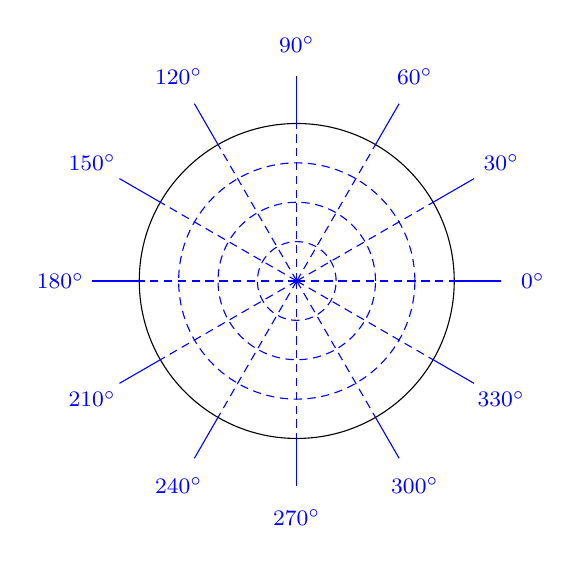
\begin{tikzpicture}[scale=2]
        \draw (0,0) circle (1);
        \foreach \i in {0, 30, ..., 330} {
            \draw[blue] ({cos(\i)},{sin(\i)}) -- ({1.3*cos(\i)},{1.3*sin(\i)});
            \draw[blue,densely dashed] (0,0) -- ({cos(\i)},{sin(\i)});
            \draw[blue] ({1.5*cos(\i)},{1.5*sin(\i)}) node {\footnotesize$\i^\circ$};
        }
        \foreach \i in {.25, .5, .75}
        {
            \draw[blue,densely dashed] (0,0) circle (\i);
        }
    \end{tikzpicture}
\end{center}

The environment's \bluett{guidelines} key may be used to display the above diagram as an overlay on the cue ball if the \bluett{\textbackslash Qty} command is present. The environment's \bluett{scale} key also affects the render of this command. We give several examples below.\medskip

\begin{minipage}{.33\linewidth}\centering
    \Qty{-.5}
    \par
    {\color{blue}\verb|\Qty{-.5};|}
\end{minipage}
\begin{minipage}{.34\linewidth}\centering
    \Qty{.33}
    \par
    {\color{blue}\verb|\Qty{.33};|}
\end{minipage}
\begin{minipage}{.33\linewidth}\centering
    \Qty[120:.75]{-.4}
    \par
    {\color{blue}\verb|\Qty[120:.75]{-.4};|}
\end{minipage}
\bigskip

\begin{minipage}{.33\linewidth}\centering
    \Qty[-90:.7]{-.1}
    \par
    {\color{blue}\verb|\Qty[-90:.7]{-.1};|}
\end{minipage}
\begin{minipage}{.34\linewidth}\centering
    \Qty[30:.25]{.8}
    \par
    {\color{blue}\verb|\Qty[30:.25]{.8};|}
\end{minipage}
\begin{minipage}{.33\linewidth}\centering
    \Qty[210:.7]{-.7}
    \par
    {\color{blue}\verb|\Qty[210:.7]{-.7};|}
\end{minipage}\bigskip

It is expected that only one \bluett{\textbackslash Qty} command is present within a given \bluett{bTable} environment. However, if multiple instances are used, no error is raised, and the corresponding diagrams are simply stacked on top of one another.

\subsection{Outside the \bluett{bTable} Environment}

The macro is still named \bluett{\textbackslash Qty}, and its syntax remains unchanged, except that it now accepts the optional \bluett{scale} and \bluett{guidelines} key–value parameters enclosed in chevrons.

\begin{minipage}{.5\linewidth}\centering
    \Qty[210:.7]{-.7}
    \par
    {\color{blue}\verb|\Qty[210:.7]{-.7}|}
\end{minipage}
\begin{minipage}{.5\linewidth}\centering
    \Qty<scale=1.5>[210:.7]{-.7}
    \par
    {\color{blue}\verb|\Qty<scale=1.5>[210:.7]{-.7}|}
\end{minipage}
\bigskip

\begin{minipage}{.5\linewidth}\centering
    \Qty<guidelines>{.75}
    \par
    {\color{blue}\verb|\Qty<guidelines>{.75}|}
\end{minipage}
\begin{minipage}{.5\linewidth}\centering
    \Qty<guidelines>[90:.7]{-.5}
    \par
    {\color{blue}\verb|\Qty<guidelines>[90:.7]{-.5}|}
\end{minipage}

\section{Tik\textit{Z} Layering}

No clipping path is applied to user-defined drawings; consequently, graphical elements may extend beyond the boundaries of the table.

The package renders elements in a fixed order: the table, the shaded areas, the user's \bluett{\textbackslash draw} commands, the box outlines, and finally the balls. This drawing order determines the visual stacking of all elements.

Internally, every \bluett{\textbackslash draw} command is stored in the \verb|\l__billiards_drawcalls_tl| token list. Likewise, shaded areas, box outlines, and balls are stored in the \verb|\l__billiards_shadedboxes_tl|, \verb|\l__billiards_boxes_tl|, and \verb|\l__billiards_balls_tl| token lists, respectively. The \verb|\l__billiards_shadedboxes_tl| token list is processed before the grid lines are drawn.

The processing order is therefore as follows:
\begin{enumerate}
    \item the table and the shaded areas;
    \item the markings (the ``mouches'', the ``ancres'', the grid lines, etc.);
    \item the \bluett{\textbackslash draw} commands;
    \item the box outlines;
    \item the billiard balls;
    \item the guidelines, if specified.
\end{enumerate}

The output of the \bluett{\textbackslash Qty} macro is processed before all items in the above list. Consequently, a \bluett{\textbackslash ShadedRegion} command will be rendered on \textit{above} the output produced by \bluett{\textbackslash Qty}.

In the event of overlapping \bluett{\textbackslash draw} commands, the corresponding drawings are rendered in the order in which the commands appear. The same principle applies to overlapping billiard balls.

\section{Future Development}

Possible areas for future development include, and are not limited to:
\begin{itemize}
    \item support for the addition of user-defined ball colours;
    \item enhanced versatility of markings and annotations;
    \item support for easy handling of curved trajectories (used in ``artistic billiards'').
\end{itemize}

These features are under consideration and may be implemented in future releases.

\section{Some Further Examples}

We present eight examples that illustrate a variety of use cases and showcase the possibilities offered by the package. Readers are warmly encouraged to try reproducing these shots on an actual billiard table.\bigskip

\begin{bTable}
    \YBall (8-2*\br,4-2*\br);
    \RBall (3,3);
    \WBall (3,1);
    \trBox;
    \draw \wpos \To \rbdry[180] \To (1.7,4) \To (0,2.5) \To (2.6,0) \To \ypos;
    \Qty[135:.7]{-.5};
    \dash \rpos -- (3.6,4) -- (5.8,0) -- (7.5,3.3);
\end{bTable}

\begin{verbatim}
\begin{bTable}
    \YBall (8-2*\br,4-2*\br);
    \RBall (3,3);
    \WBall (3,1);
    \trBox;
    \draw \wpos \To \rbdry[180] \To (1.7,4) \To (0,2.5) \To (2.6,0) \To \ypos;
    \Qty[135:.7]{-.5};
    \dash \rpos -- (3.6,4) -- (5.8,0) -- (7.5,3.3);
\end{bTable}
\end{verbatim}

\begin{bTable}
    \YBall (2*\br,2*\br);
    \WBall (2,.5);
    \RBall (5,.5);
    \blBox;
    \draw \wpos \To \rbdry[90] \To (8,2.7) \To (6.2,4) \To \ypos;
    \dash \rpos -- (5.6,0) -- (8,1.7) -- (5.4,4) -- (.5,.7);
    \Qty[90:.7]{-.5};
\end{bTable}

\begin{verbatim}
\begin{bTable}
    \YBall (2*\br,2*\br);
    \WBall (2,.5);
    \RBall (5,.5);
    \blBox;
    \draw \wpos \To \rbdry[90] \To (8,2.7) \To (6.2,4) \To \ypos;
    \dash \rpos -- (5.6,0) -- (8,1.7) -- (5.4,4) -- (.5,.7);
    \Qty[90:.7]{-.5};
\end{bTable}
\end{verbatim}

\begin{bTable}
    \WBall (1.5,4-3*\br);
    \RBall (2,4-3*\br);
    \YBall (3*\br,3*\br);
    \draw \wpos -- \rbdry[135] -- (1.8,4) \To \ypos;
    \dash \rpos -- (8,2.3) -- (.8,.3);
    \ShadedRegion (0,0) -- (1,1);
    \Qty[-90:.7]{-.5};
\end{bTable}

\begin{verbatim}
\begin{bTable}
    \WBall (1.5,4-3*\br);
    \RBall (2,4-3*\br);
    \YBall (3*\br,3*\br);
    \draw \wpos -- \rbdry[135] -- (1.8,4) \To \ypos;
    \dash \rpos -- (8,2.3) -- (.8,.3);
    \ShadedRegion (0,0) -- (1,1);
    \Qty[-90:.7]{-.5};
\end{bTable}
\end{verbatim}

\begin{bTable}
    \WBall (.5,3);
    \RBall (1+\br,3+\br);
    \YBall (3*\br,3*\br);
    \draw \wbdry[0] \To \rbdry[-135] \To \ypos;
    \dash \rpos -- (4.8,4) -- (8,3.1) -- (.8,.5);
    \ShadedRegion (0,0) -- (1,1);
    \Qty[-90:.7]{.25};
\end{bTable}

\begin{verbatim}
\begin{bTable}
    \WBall (.5,3);
    \RBall (1+\br,3+\br);
    \YBall (3*\br,3*\br);
    \draw \wbdry[0] \To \rbdry[-135] \To \ypos;
    \dash \rpos -- (4.8,4) -- (8,3.1) -- (.8,.5);
    \ShadedRegion (0,0) -- (1,1);
    \Qty[-90:.7]{.25};
\end{bTable}
\end{verbatim}

\begin{bTable}
    \WBall (6,2);
    \RBall (2,3);
    \YBall (3,3*\br);
    \draw \wpos \To \rbdry[-90] \To (0,1.9) \To \ypos;
    \dash \rpos -- (1.1,4) -- (0,2.9) -- (2.7,.6);
    \Box (2.5,0) -- (4.2,1);
    \Qty[90:.7]{-.5};
\end{bTable}

\begin{verbatim}
\begin{bTable}
    \WBall (6,2);
    \RBall (2,3);
    \YBall (3,3*\br);
    \draw \wpos \To \rbdry[-90] \To (0,1.9) \To \ypos;
    \dash \rpos -- (1.1,4) -- (0,2.9) -- (2.7,.6);
    \Box (2.5,0) -- (4.2,1);
    \Qty[90:.7]{-.5};
\end{bTable}
\end{verbatim}

\begin{bTable}
    \RBall (2,2);
    \WBall (1.5,1.75);
    \YBall (.25,.25);
    \draw \wpos -- \rbdry[150] \To (1.5,4) \To (.25,.25);
    \dash \rpos -- (8,1.5) -- (.5,.5);
    \blBox;
    \Qty[-135:.75]{-.9};
\end{bTable}

\begin{verbatim}
\begin{bTable}
    \RBall (2,2);
    \WBall (1.5,1.75);
    \YBall (.25,.25);
    \draw \wpos -- \rbdry[150] \To (1.5,4) \To (.25,.25);
    \dash \rpos -- (8,1.5) -- (.5,.5);
    \blBox;
    \Qty[-135:.75]{-.9};
\end{bTable}
\end{verbatim}

\begin{bTable}
    \RBall (6,2);
    \YBall (2,2);
    \WBall (2,1.5);
    \Qty[60:.75]{-.5};
    \draw \wpos \To \rbdry[90] \To (7.7,4) -- (8,3.8) \To (5.2,0) \To \ypos;
    \dash \rpos -- (8,1.2) -- (3.7,0) -- (.5,.6);
    \ShadedRegion (0,0) -- (8/3,4);
\end{bTable}

\begin{verbatim}
\begin{bTable}
    \RBall (6,2);
    \YBall (2,2.5);
    \WBall (2,1.5);
    \Qty[60:.75]{-.5};
    \draw \wpos \To \rbdry[90] \To (7.7,4) -- (8,3.8) \To (5.2,0) \To \ypos;
    \dash \rpos -- (8,1.2) -- (3.7,0) -- (.5,.6);
    \ShadedRegion (0,0) -- (8/3,4);
\end{bTable}
\end{verbatim}

\begin{bTable}
    \YBall (1,4-\br);
    \RBall (2,2);
    \WBall (1.5,2.15);
    \Qty[300:.7]{-.1};
    \draw \wpos -- \rbdry[150] \To (0,2.9) \To \ypos;
    \ShadedRegion (0,2) -- (2,4);
    \dash \rpos -- (7.3,0) -- (8,.3) -- (1.5,3.7);
\end{bTable}

\begin{verbatim}
\begin{bTable}
    \YBall (1,4-\br);
    \RBall (2,2);
    \WBall (1.5,2.15);
    \Qty[300:.7]{-.1};
    \draw \wpos -- \rbdry[150] \To (0,2.9) \To \ypos;
    \ShadedRegion (0,2) -- (2,4);
    \dash \rpos -- (7.3,0) -- (8,.3) -- (1.5,3.7);
\end{bTable}
\end{verbatim}

\end{document}